% !TeX spellcheck = en_US
\documentclass[french]{yLectureNote}

\title{Atomistique 2 - PS}
\subtitle{Chimie}
\author{Paulhenry Saux}
\date{\today}
\yLanguage{Français}

\professor{J.Cunny}
\usepackage{graphicx}%----pour mettre des images
\usepackage[utf8]{inputenc}%---encodage
\usepackage{geometry}%---pour modifier les tailles et mettre a4paper
%\usepackage{awesomebox}%---pour les boites d'exercices, de pbq et de croquis ---d\'esactiv\'e pour les TP de PC
\usepackage{tikz}%---pour deiffner + d\'ependance de chemfig
% \usepackage{tabularx}%---pour dimensionner automatiquement les tableaux avec variable X
\usepackage{awesomebox}%---Pour les boites info, danger et autres
\usepackage{menukeys}%---Pour deiffner les touches de Calculatrice
\usepackage{fancyhdr}%---pour les en-t\^ete personnalis\'ees
\usepackage{blindtext}%---pour les liens
\usepackage{hyperref}%---pour les liens (\`a mettre en dernier)
\usepackage{caption}%---pour la francisation de la l\'egende table vers Tableau
\usepackage{pifont}
\usepackage{array}%---pour les tableaux
\usepackage{lipsum}
\usepackage{yFlatTable}
\usepackage{multicol}
\newcommand{\Lim}[1]{\lim\limits_{\substack{#1}}\:}
\renewcommand{\vec}{\overrightarrow}
\newcommand{\N}[0]{\mathbb{N}}
\newcommand{\dd}{\mathrm{d}}
\newcommand{\norm}[1]{||\vec{#1}||}
\newcommand{\fo}{\psi(\vec{r},t)}
\newcommand{\foe}{\psi(\vec{r},t)\*}
\newcommand{\HH}{\hat{H}}
\newcommand{\hb}{\hbar}
\newcommand{\lap}{\nabla^2}
\newcommand{\lapcc}{\frac{\partial^2 }{\partial x^2}+\frac{\partial^2 }{\partial y^2}+\frac{\partial^2 }{\partial z^2}}
\begin{document}
\setcounter{chapter}{2}
\chapter{Méthode Huckel}
\section{Principe}
On se place dans les approximations de BO, orbitales et LCAO.

On veut toujours résoudre ce système
\[
\begin{bmatrix}
h_{11} & h_{12} & \cdots & h_{1n} \\
h_{21} & h_{22} & \cdots & h_{2n} \\
\vdots & \vdots & \ddots & \vdots \\
h_{n1} & h_{n2} & \cdots & h_{nn}
\end{bmatrix}
\begin{bmatrix}
c_1 \\
c_2 \\
\vdots \\
c_n
\end{bmatrix}
= \epsilon
\begin{bmatrix}
S_{11} & S_{12} & \cdots & S_{1n} \\
S_{21} & S_{22} & \cdots & S_{2n} \\
\vdots & \vdots & \ddots & \vdots \\
S_{n1} & S_{n2} & \cdots & S_{nn}
\end{bmatrix}
\begin{bmatrix}
c_1 \\
c_2 \\
\vdots \\
c_n
\end{bmatrix}
\]

On calcule les \(S_{ij}\) avec la formule de Wolsberg de façon numérique. Les matrices sont alors totalement définies avec cette résolution numérique
\section{Méthode simple}
\subsection{Introduction}
La méthode ne s'applique qu'à l'intéraction entre OA identiriques, portées par des atomes identiques avec une OA par atome. Ainsi,
\begin{itemize}
 \item les \(h_{ii}\) sont identiques et notés \(\alpha < 0\)
 \item les \(h_{ij}\) valent :
 \begin{itemize}
  \item 0 si les 2 OA sont non adjacentes\marginTips{i.e. séparées par au moins deux liaisons}
  \item \(\beta <0\) si les 2 OA sont adjacentes\marginTips{i.e. portées par deux atomes liés par une liaison \(\sigma\)}
 \end{itemize}
\item \(S_{ii} = 1, S_{ij} = 0 \)
\end{itemize}
\subsection{Exemples}
\subsubsection{Éthylène ($\pi$)}
On veut appliquer la méthode au système \(\pi\) de l'éthylène. L'orbitale moléculaire est une combinaison linéaire des OA 2p des atomes de carbone avec des coefficients: \[\psi = \c_1\phi_1+c_2\phi_2\]
En introduisant cette expression dans l'équation de Scrodinger puis en multipliant \(\phi_1\) et \(\phi_2\), on obtient \[ \left\{\begin{matrix}
c_1(h_{11}-\epsilon S_{11}) + c_2(h_{12}-\epsilon S_{12}) = 0\\
c_1(h_{21}-\epsilon S_{21}) + c_2(h_{22}-\epsilon S_{22}) = 0
\end{matrix}\right.\] Or, en appliquant les principes définis ci-dessus, on obtient
\[ \left\{\begin{matrix}
c_1(\alpha-\epsilon) + c_2(\beta) = 0\\
c_1(\beta) + c_2(\alpha-\epsilon ) = 0
\end{matrix}\right.\]
En mettant sous forme matricielle et en calculant le déterminant\marginWarning{On aurait aussi pu poser \(x = \frac{\alpha-\epsilon}{\beta}\) et trouver \(x=\pm 1\), ce qui revient au m\^eme}, on trouve \[ \left\{\begin{matrix}
\epsilon^+ &=\alpha+\beta\\
\epsilon^-&=\alpha-\beta
\end{matrix}\right.\]
En injectant dans le premier système d'équation, on en déduit que \(c_1 = \pm c_2\) Après normalisation\marginTips{qui revient à résoudre \(c_1^2+c_2^2 =1\)}, on trouve :
\[ \left\{\begin{matrix}
\phi^+ = \pm \frac{1}{\sqrt{2}}(\chi_1+\chi_2)\\
\phi^- = \frac{1}{\sqrt{2}}(\chi_1-\chi_2)
\end{matrix}\right.\]
Comme \(\beta <0\), on trouve le DOM suivant :
%TODO DOM à dessiner page 34
\warningInfo{Différence}{Par rapport à la dioganalisation complète, on remarque ici que l'énergie de stabilisation et de destabilisation \(\beta\) sont les m\^emes, ce qui n'est pas le cas dans la méthode exacte}
\subsubsection{Butadiene ($\pi$) }
Il y a 4 atomes, donc on obtient le système, en posant \(x = \frac{\alpha-\epsilon}{\beta}\) :
\[\begin{vmatrix}
x & 1 & 0 & 0 \\
1 & x & 1 & 0 \\
0 & 1 & x & 1 \\
0 & 0 & 1 & x \\
\end{vmatrix}\]
En développant la matrice, on trouve \[x(x(x^2-1)-x)-(x^2-1)+0 = x^4-3x^2+1\] que l'on peut résoudre en posant \(X = x^2\). On a alors
\[\left\{\begin{matrix}
X_1 = \frac{3+\sqrt{5}}{2}\\
X_2 = \frac{3-\sqrt{5}}{2}
\end{matrix}\right.
\Rightarrow
\left\{\begin{matrix}
x_1 = +\frac{3+\sqrt{5}}{2}\\
x_2 = +\frac{3-\sqrt{5}}{2}\\
x_3 = -\frac{3+\sqrt{5}}{2}\\
x_4 = -\frac{3-\sqrt{5}}{2}
\end{matrix}\right.
\Rightarrow
\left\{\begin{matrix}
\epsilon_1 = \alpha-\frac{3+\sqrt{5}}{2}\beta \simeq \alpha - 1.618\beta\\
\epsilon_2 = \alpha-\frac{3-\sqrt{5}}{2}\beta \simeq \alpha - 0.618\beta \\
\epsilon_3 = \alpha+\frac{3+\sqrt{5}}{2}\beta \simeq \alpha + 0.618\beta\\
\epsilon_4 = \alpha+\frac{3-\sqrt{5}}{2}\beta \simeq \alpha + 1.618\beta
\end{matrix}\right.
\]

Maintenant que nous connaissons \(x\), on peut résoudre le système d'équation original pour trouver les constantes :
\[\left\{\begin{matrix}
xc_1+c_2=0\\
c_1+xc_2+c_3=0\\
c_2+xc_3+c_4=0\\
c_3+xc_4=0
\end{matrix}\right.\]
On trouve que \(c_1=c_4, c_2=c_3, c_1 = -(x+1)c_2, xc_1=-c_2\)\marginCritical{Pour les trouver, il est nécessaire d'effectuer des considérations de symétrie sur les OM de la molécule} pour en déduire que \(1.618c_1=c_2=c_3\). Les OM\marginCritical{Les coefficients devant les OA ont une influence sur la taille des OM à dessiner et sur leur signe !} sont donc\marginTips{Trouvée avec normalisation} \[
\left\{\begin{matrix}
\pi_1 = 0.372\chi_1+0.602\chi_2+0.602\chi_3+0.373\chi_4\\
\pi_2 = 0.602\chi_1+0.372\chi_2-0.602\chi_3-0.602\chi_4\\
\pi_3 = 0.602\chi_1-0.372\chi_2-0.602\chi_3+0.602\chi_4\\
\pi_4 = 0.372\chi_1-0.602\chi_2+0.602\chi_3-0.373\chi_4\\
\end{matrix}\right.
\]

\includegraphics[scale=0.5]{figures/but}
\subsubsection{H3 trigonal}
Les 3 atomes d'hydrogène sont liés entre eux : c'est une strycture cyclique. Il faut donc trouver le déterminant de \[\begin{vmatrix}
x&1&1\\
1&x&1\\
1&1&x
\end{vmatrix} = (x-1)^(x+2)\] On remarque qu'il y a une racine double. Il y aura donc 2 OM dégénérées au niveau d'énergie \(\alpha-1\beta\).

Commençon par l'OM du niveau \(\alpha+2\beta\) en replaçant \(x\) par sa valeur \(-2\). On a le système \[\left\{\begin{matrix}
-2c_1+c_2+c_3=0\\
c_1-2c_2+c_3=0\\
c_1+c_2-2c_3=0
\end{matrix}\right.\] qui donne \(c_1=c_2=c_3\)\marginInfo{On peut déjà remarquer que les OA de l'OM seront de m\^eme taille car les coefficients sont égaux}. On applique la condiion de normalisation sur \(\phi_1 = c_1(\chi_1+\chi_2+\chi_3)\) pour trouver \(c_1 = \pm \frac{1}{\sqrt{3}}\).

Trouvons maintenant \(\phi_2\), une des OM dégénérées du niveau \(\alpha-1\beta\). La résolution du système conduit à \(c_1+c_2+c_3 =0\). Comme on est en présence d'OM dégénérées, on peut mettre un coefficient à nul, ici on choisit \(c_1 = 0\). On obtient ainsi \(c_2=-c_3\). On a ainsi \[\phi_2 = c_2(\chi_2-\chi_3)\]La conditon de normalisation donne \(c_2 = \pm \frac{1}{\sqrt{2}}\).

Pour trouver la seconde OM dégénérée, on ne peut pas mettre \(c_2\) ou \(c_3\) à 0 car on trouverait la m\^eme OM. On va utiliser la propriété d'orthogonalité des OM avec \(\phi_2\) et \(\phi_1\).


\begin{align*}
\langle \phi_3 | \phi_2 \rangle &= \left\langle \pm \frac{1}{\sqrt{2}}(\chi_2 - \chi_3) \bigg| c_1\chi_1 + c_2\chi_2 + c_3\chi_3 \right\rangle \\
&= \pm \frac{1}{\sqrt{2}} \left[ c_1\langle\chi_2|\chi_1\rangle + c_2\langle\chi_2|\chi_2\rangle + c_3\langle\chi_2|\chi_3\rangle - c_1\langle\chi_3|\chi_1\rangle - c_2\langle\chi_3|\chi_2\rangle - c_3\langle\chi_3|\chi_3\rangle \right] \\
&= \pm \frac{1}{\sqrt{2}} \left[ c_1(0) + c_2(1) + c_3(0) - c_1(0) - c_2(0) - c_3(1) \right] \\
&= \pm \frac{1}{\sqrt{2}} (c_2 - c_3)
\end{align*}
La condition est donc $c_2 = c_3$.

Pour la seconde condition d'orthogonalité :

\begin{align*}
\langle \phi_1 | \phi_3 \rangle &= \left\langle \pm \frac{1}{\sqrt{3}}(\chi_1+\chi_2+\chi_3) \bigg| c_1\chi_1+c_2\chi_2+c_2\chi_3 \right\rangle \\
&= \pm \frac{1}{\sqrt{3}} \left[ c_1\langle\chi_1|\chi_1\rangle + c_2\langle\chi_1|\chi_2\rangle + c_2\langle\chi_1|\chi_3\rangle \right. \\
& \quad + \left. c_1\langle\chi_2|\chi_1\rangle + c_2\langle\chi_2|\chi_2\rangle + c_2\langle\chi_2|\chi_3\rangle \right. \\
& \quad + \left. c_1\langle\chi_3|\chi_1\rangle + c_2\langle\chi_3|\chi_2\rangle + c_2\langle\chi_3|\chi_3\rangle \right] \\
&= \pm \frac{1}{\sqrt{3}} \left[ c_1(1) + c_2(1) + c_2(1) \right] \\
&= \pm \frac{1}{\sqrt{3}}(c_1 + 2c_2)
\end{align*}
La condition est donc $c_1 = -2c_2$.


On trouve ainsi \(c_2 = c_3, c_1 = -2c_2\). Avec la condition de normalisation, on obtient \(c_2 = \pm \frac{1}{\sqrt{6}}\)
Donc \[\phi_3 = \pm \frac{1}{\sqrt{6}}(-2\chi_1+\chi_2+\chi_3)\]
%DOM TODO page 74
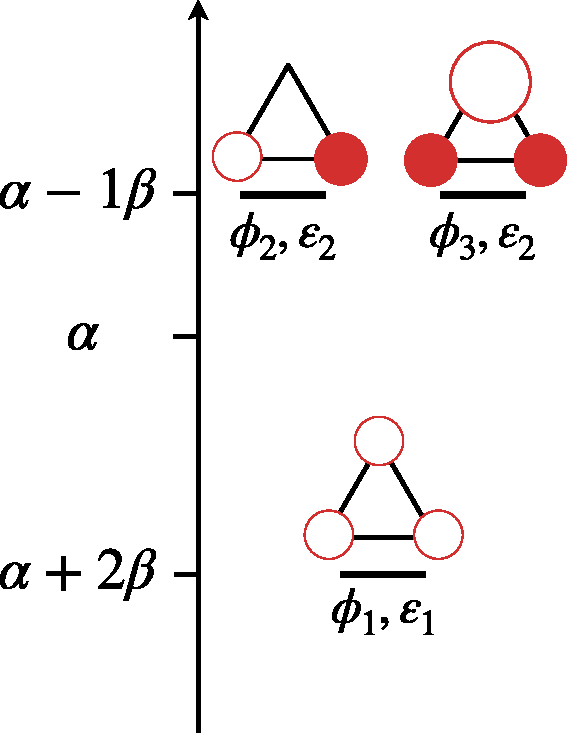
\includegraphics[scale=0.5]{figures/trigo}
\subsubsection{H4 Carré plan}
On cherche le déterminant de \[\begin{vmatrix}
x & 1 & 0 & 1 \\
1 & x & 1 & 0 \\
0 & 1 & x & 1 \\
1 & 0 & 1 & x \\
\end{vmatrix}\] On obtient \[x^2(x-2)(x+2)\] On aura donc 2 OA dégénérées au niveau \(\alpha\), une au niveau \(\alpha-2\beta\) et une au niveau \(\alpha+2\beta\)

Cherchons \(\phi_1\) pour \(x=-2\). En injectant dans le système, on trouve \(c_1=c_2=c_3=c_4\). Donc \(\phi_1 = c_1(\chi_1+\chi_2+\chi_3+\chi_4)\). La condition de normalisation donne \(c_1 = \frac{1}{\sqrt{4}}\), donc \[\phi_1 = \pm \frac{1}{2}(\chi_1+\chi_2+\chi_3+\chi_4)\]

Cherchons \(\phi_3\). En injectant \(x=2\), trouve \(c_1=-c_2=c_3=-c_4\). Donc avec la condition de normalisation, on obtient \[\phi_4 = \pm \frac{1}{2}(\chi_1-\chi_2+\chi_3-\chi_4)\]

Cherchons maintenant \(\phi_2\). Avec \(x=0\), on a \(c_2=-c_4, c_1=-c_3\). Les OM sont dégénérées, on peut donc supposer \(c_2 = -c_4 = 0\). Ainsi, \(\phi_1 = c_1-\chi_1-\chi_3\). Finalement \[\phi_2 = \pm \frac{1}{\sqrt{2}}(\chi_1-\chi_3)\]

Pour la dernière, on a \(\phi_3 = c_1\chi_1+c_2\chi_2-c_1\chi_3-c_2\chi_4\). On se sert de la condition d'orthogonalité avec \(\phi_2\) :

\begin{align*}
\langle \phi_2 | \phi_3 \rangle &= \left\langle \pm \frac{1}{\sqrt{2}}(\chi_1-\chi_3) \bigg| c_1\chi_1+c_2\chi_2-c_1\chi_3-c_2\chi_4 \right\rangle \\
&= \pm \frac{1}{\sqrt{2}} \left[ c_1\langle\chi_1|\chi_1\rangle + c_2\langle\chi_1|\chi_2\rangle - c_1\langle\chi_1|\chi_3\rangle - c_2\langle\chi_1|\chi_4\rangle \right. \\
& \quad - \left. c_1\langle\chi_3|\chi_1\rangle - c_2\langle\chi_3|\chi_2\rangle - (-c_1)\langle\chi_3|\chi_3\rangle - (-c_2)\langle\chi_3|\chi_4\rangle \right] \\
&= \pm \frac{1}{\sqrt{2}} [ c_1(1) - (-c_1)(1) ] \\
&= \pm \frac{1}{\sqrt{2}}(c_1+c_1) \\
&= \pm \frac{1}{\sqrt{2}}(2c_1) \\
&= \pm \sqrt{2}c_1
\end{align*}
La condition est donc $c_1 = 0$. Avec la condition de normalisation, on a \[\phi_3 = \pm \frac{1}{\sqrt{2}}(\chi_2-\chi_4)\]

\includegraphics[scale=0.5]{figures/carre_plan}
 \end{document}
